
\newpage

%=================================================[SECTION: One Dimensional Systems]
\subsection{ONE DIMENSIONAL SYSTEMS} 

In order to further illustrate the non-linear forecasting technique and the deterministic metric, two different one dimensional systems with different underlying dynamics are analyzed under verying amplitudes of noise. The first is the logistic map,

$$X_{t+1} = r X_t (1-X_t) + \alpha\eta,$$
where $r$ is a parameter of the system, $\alpha$ is the amplitude of the noise, and $\eta$ is uncorrelated noise with values between 0 and 1. For certain values of $r$ and zero noise ($\alpha=0$), the map produces deterministic chaos \cite{logistic_equation}. The addition of varying amplitudes of noise (Figure \ref{logistic_noise}) does not seem to change the qualitative appearance of the resulting time series. 

\begin{figure}[htbp]  %FIGURE
   \centering
   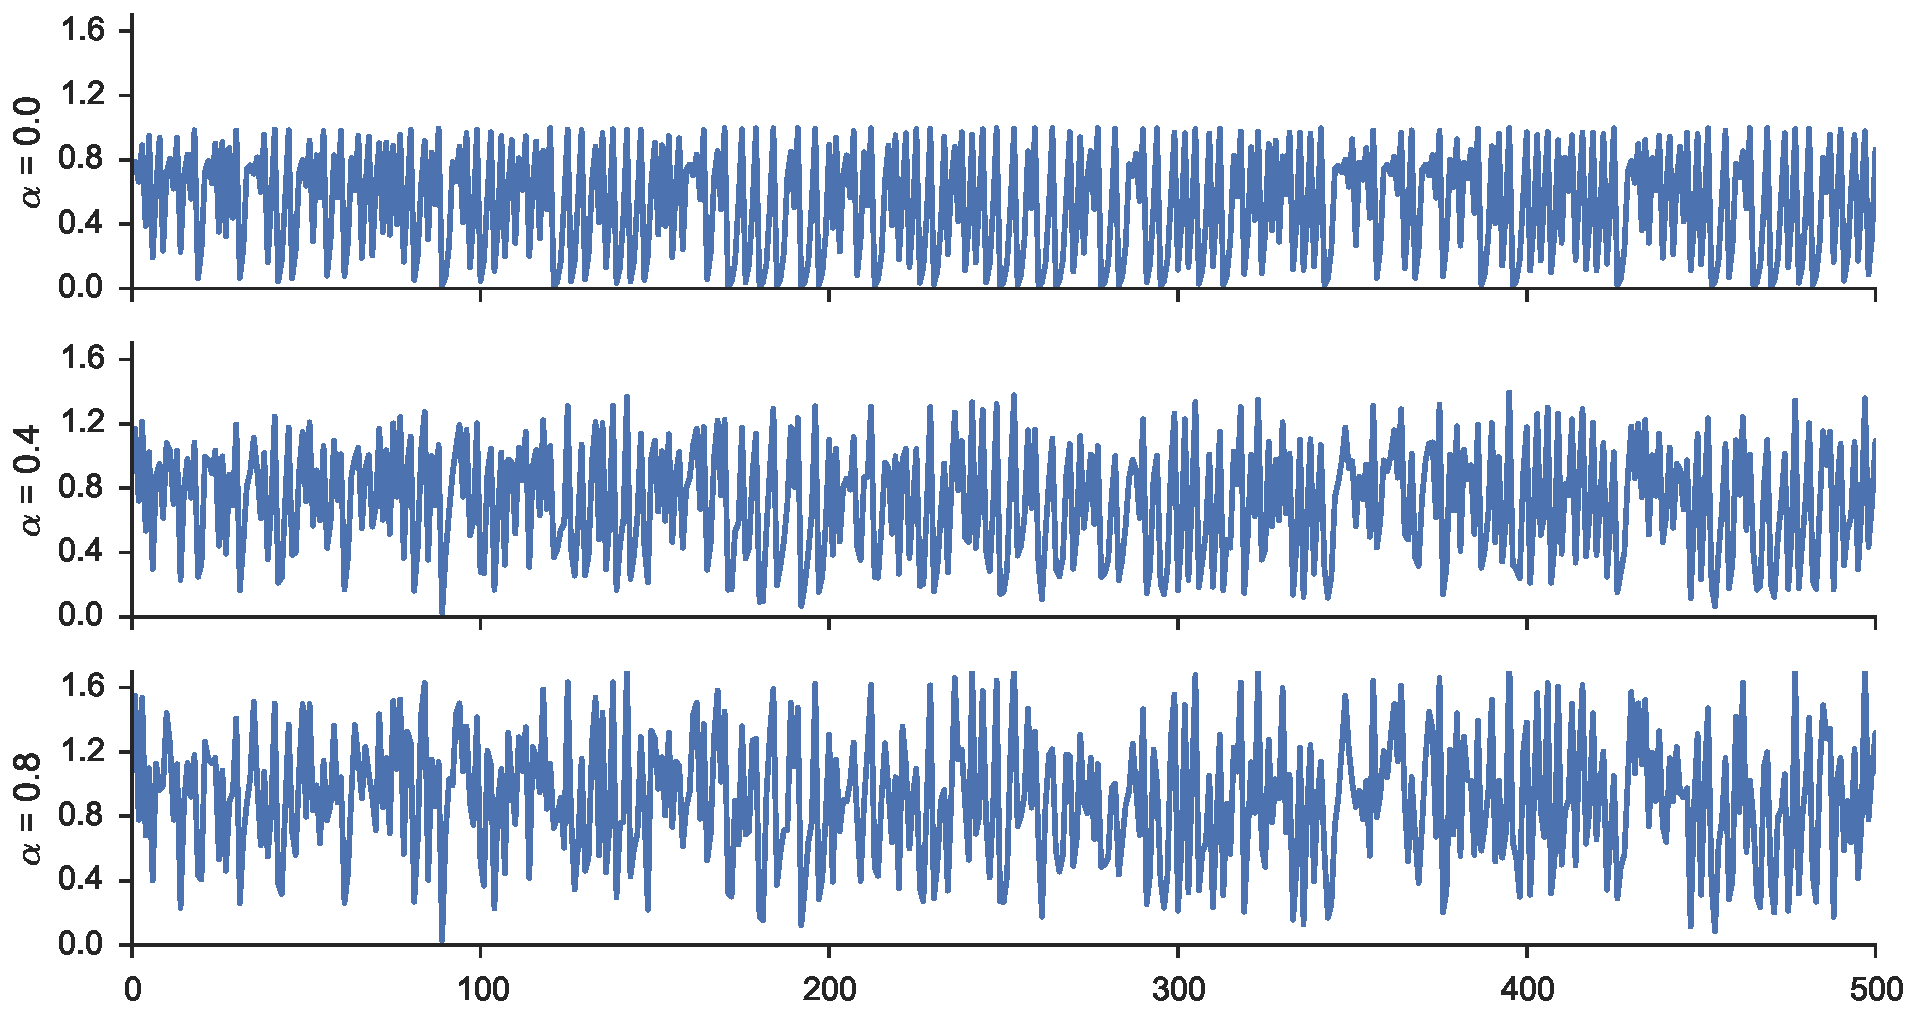
\includegraphics[width=4 in]{1d/logistic_noise.pdf} 
   \caption{Time series from the logistic map with different amplitudes of noise as indicated by $\alpha$. }
   \label{logistic_noise}
\end{figure}


Next a periodic function with noise added,

$$X(t) = sin(t) +\frac{1}{2}cos(t) + \frac{1}{4}sin(\frac{1}{4}t) + \alpha\eta,$$
is used to generate a number of different time series with various amplitudes of noise for analysis (Figure \ref{periodic_noise}).

\begin{figure}[htbp]  %FIGURE
   \centering
   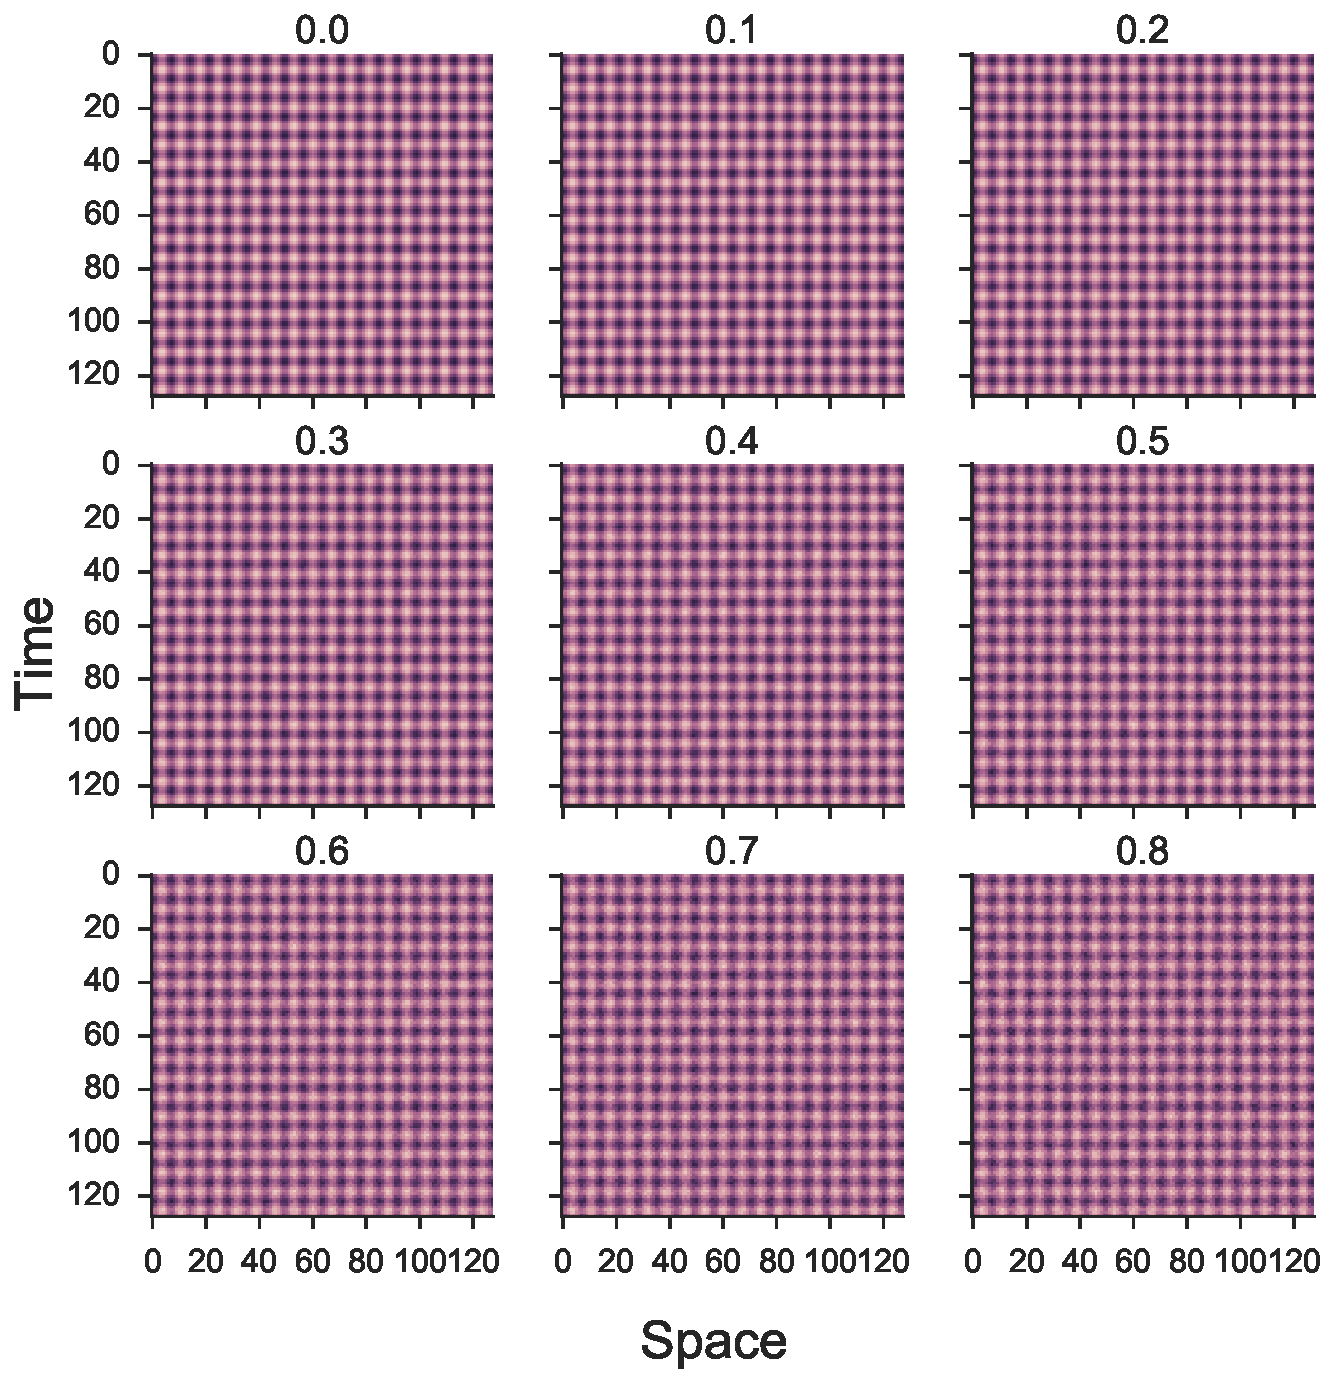
\includegraphics[width=4 in]{1d/periodic_noise.pdf} 
   \caption{Time series resulting from the periodic equation with different amplitudes of noise as indicated by $\alpha$.}
   \label{periodic_noise}
\end{figure}


The non-linear forecasting technique is applied to both systems (Figure \ref{logistic_contours}) and (Figure \ref{periodic_contours}) for nine different amplitudes of noise added to each system.


\begin{figure}[htbp]  %FIGURE
   \centering
   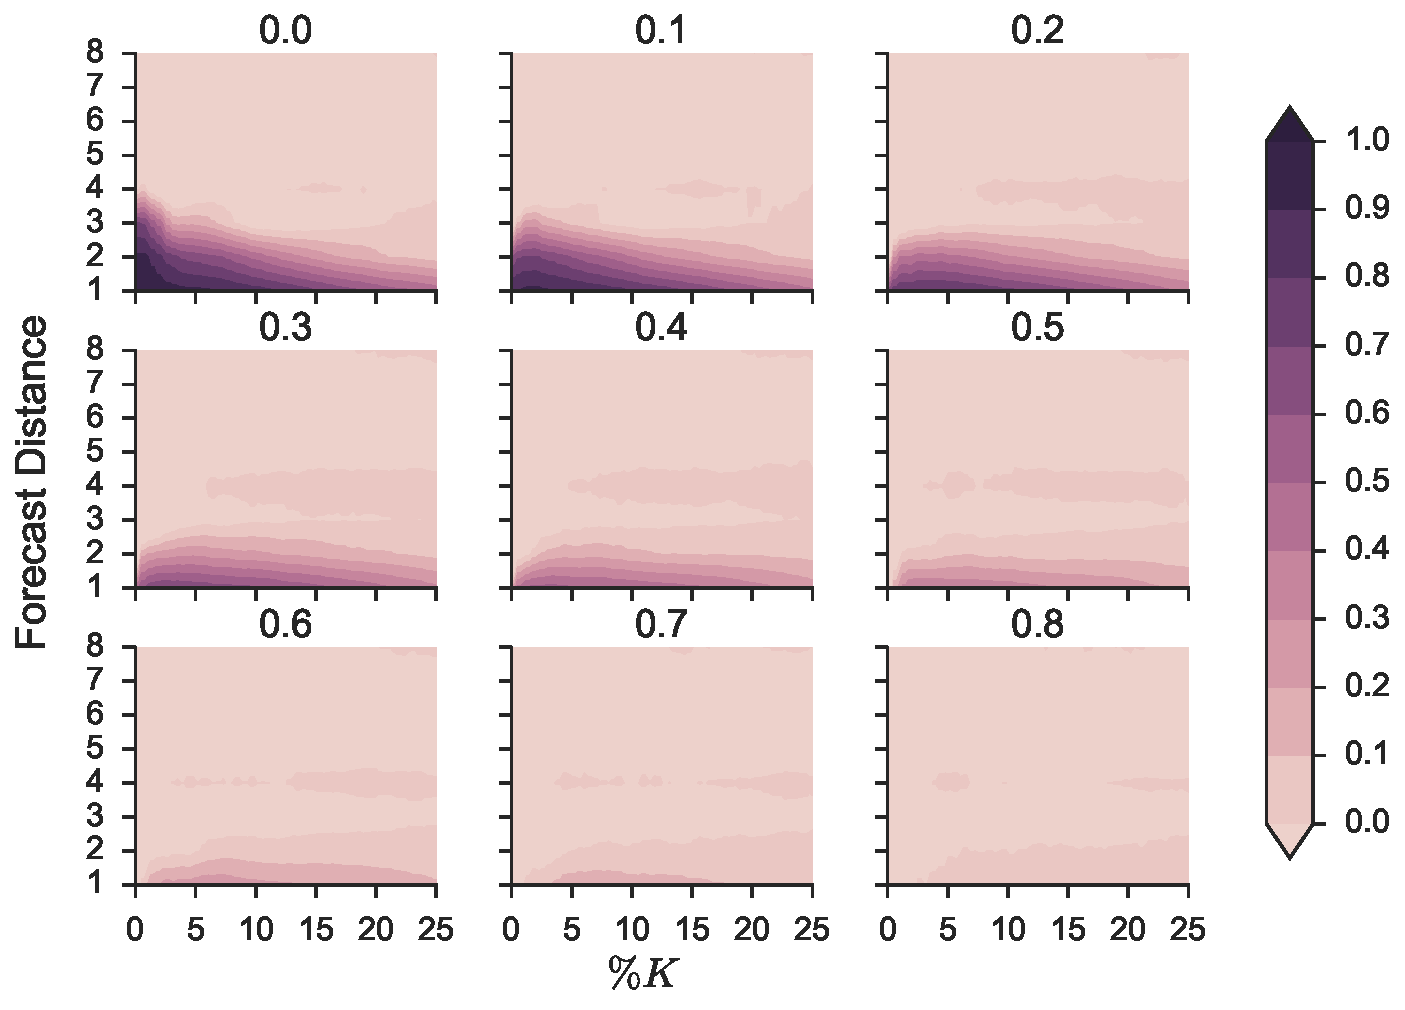
\includegraphics[width=4 in]{1d/chaotic_contours.pdf} 
   \caption{Non-linear forecasting results for the logistic map with different amplitudes of noise. The coefficient of determination, $R^2$, is plotted against near neighbors ($K$) and forecast distance. Title corresponds to the amplitude of the noise, $\alpha$.}
   \label{logistic_contours}
\end{figure}



\begin{figure}[htbp]  %FIGURE
   \centering
   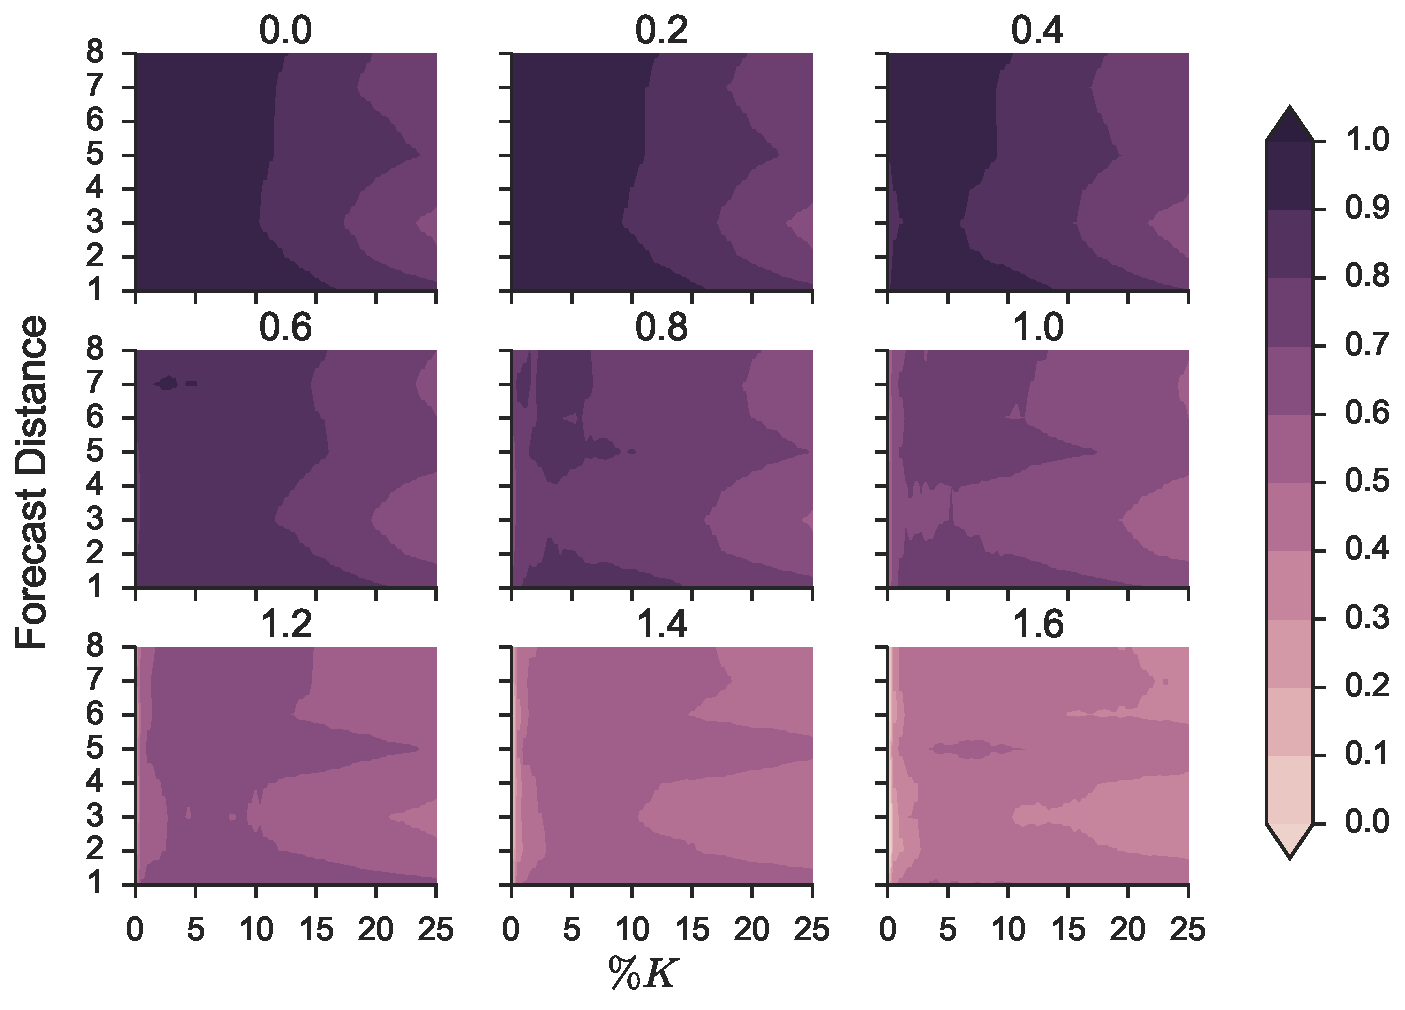
\includegraphics[width=4 in]{1d/periodic_contours.pdf} 
   \caption{Non-linear forecasting results for the periodic equation with different amplitudes of noise. The coefficient of determination, $R^2$, is plotted against near neighbors ($K$) and forecast distance. Title corresponds to the amplitude of the noise, $\alpha$.}
   \label{periodic_contours}
\end{figure}

The results from the non-linear forecasting technique illustrate the different underlying dynamics of each system. For the periodic equation, the $R^2$ values do not decrease with increasing forecasting distance and they do not decrease as rapidly as the logistic map with increasing near neighbors used.  The system simply repeats its behavior and thus forecasting is trivial.  Moreover, the reconstructed state space for the periodic equation is geometrically less complex than the logistic map (Figure \ref{phase_spaces}). This allows a greater percent of near neighbor trajectories to be averaged before $R^2$ values start to decrease.

The analysis of the logistic map time series displays the same trends as the forecasting results from the Lorenz time series. High $R^2$ values at low values of $K$ and low forecast distance reveals the system's locality of phase space dynamics and sensitivity to initial conditions. 

\begin{figure}[htbp]  %FIGURE
   \centering
   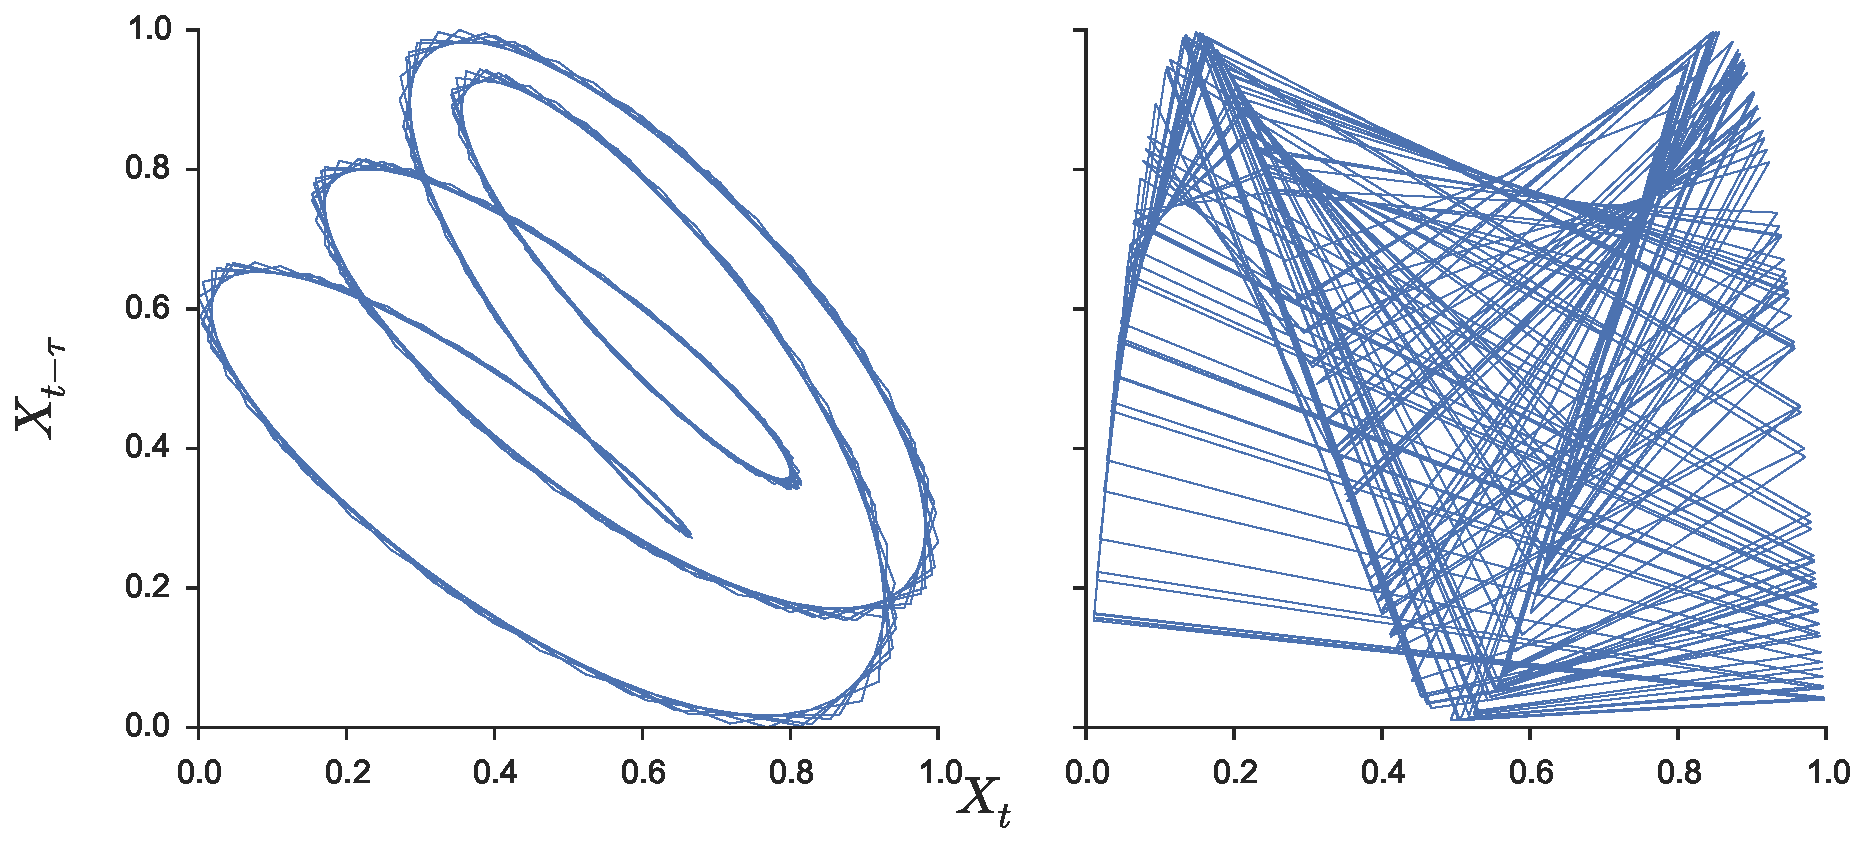
\includegraphics[width=4 in]{1d/periodic_and_chaos_embedded.pdf} 
   \caption{Two-dimensional reconstructions of the phase space for the periodic equation (left panel) and the logistic map (right panel) with lag values found from the first minimum in the mutual information.}
   \label{phase_spaces}
\end{figure}


The deterministic metric is calculated for both the logistic and periodic systems and the results are shown in Figure \ref{logistic_bar_plot} and Figure \ref{periodic_bar_plot} respectively.



\begin{figure}[htbp]  %FIGURE
   \centering
   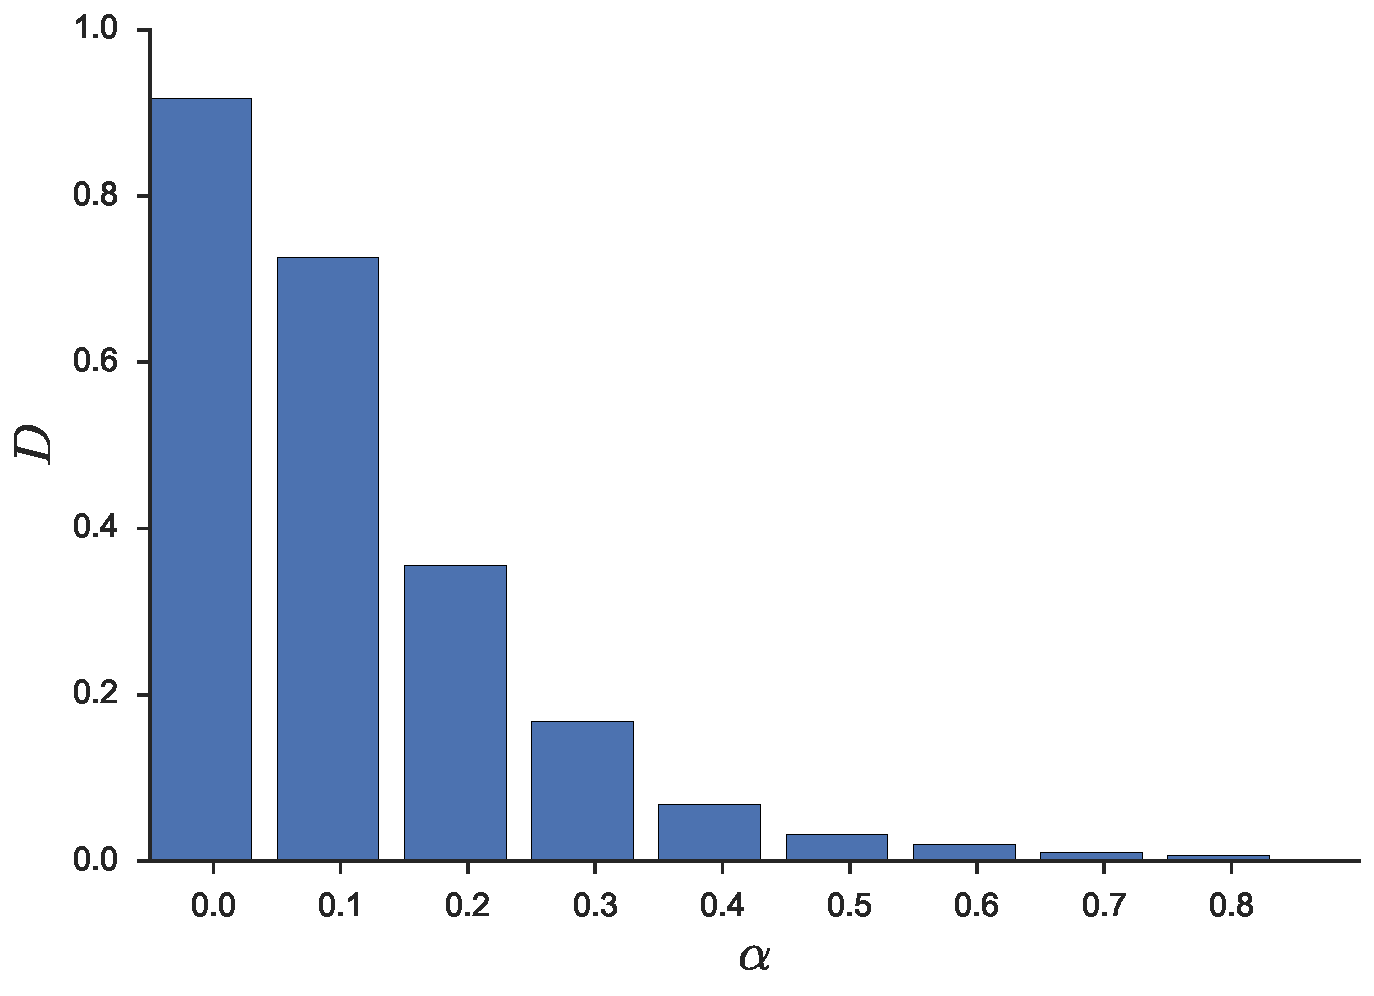
\includegraphics[width=4 in]{1d/chaotic_bar_plot.pdf} 
   \caption{Deterministic metric for the logistic map  with varying amplitudes, $\alpha$ of added noise.}
   \label{logistic_bar_plot}
\end{figure}

\begin{figure}[htbp]  %FIGURE
   \centering
   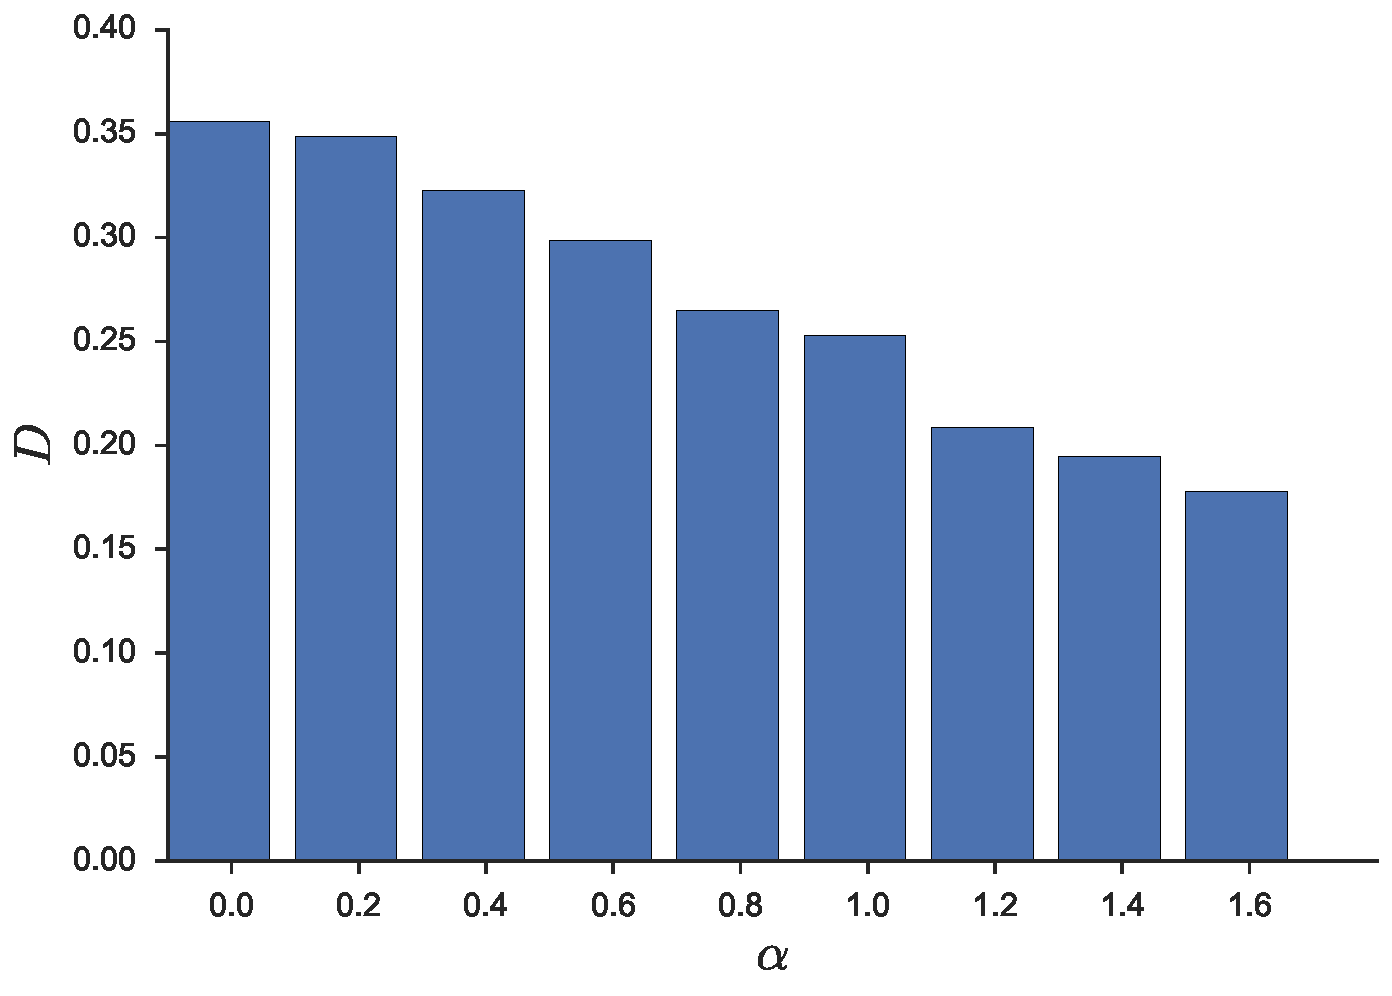
\includegraphics[width=4 in]{1d/periodic_bar_plot.pdf} 
   \caption{Deterministic metric for the periodic equation with varying amplitudes, $\alpha$ of added noise.}
   \label{periodic_bar_plot}
\end{figure}



The deterministic metric is able to distinguish the relative level of noise in the logistic map time series.  This is again because the metric captures the benefit to using local neighbors in the reconstructed phase space and as noise is added to the system, the importance of localized phase space dynamics is reduced.  Additionally, when sufficiently high amounts of noise are present in the system(e.g., the logistic map with noise levels between 0.7-0.9) it becomes difficult to distinguish the relative determinism.  The overall low forecast skill masks determinism in the system's state space. For the periodic system, since there is minimal benefit to using localized neighbors in forecasting even with low levels of noise, the deterministic metric shows a smaller reduction as noise is added to the system.  Hence, the metric is capturing determinism that results from localized, or nonlinear, dynamics in the phase space.  









